%
% File acl2015.tex
%
% Contact: car@ir.hit.edu.cn, gdzhou@suda.edu.cn
%%
%% Based on the style files for ACL-2014, which were, in turn,
%% Based on the style files for ACL-2013, which were, in turn,
%% Based on the style files for ACL-2012, which were, in turn,
%% based on the style files for ACL-2011, which were, in turn, 
%% based on the style files for ACL-2010, which were, in turn, 
%% based on the style files for ACL-IJCNLP-2009, which were, in turn,
%% based on the style files for EACL-2009 and IJCNLP-2008...

%% Based on the style files for EACL 2006 by 
%%e.agirre@ehu.es or Sergi.Balari@uab.es
%% and that of ACL 08 by Joakim Nivre and Noah Smith

\documentclass[11pt]{article}
\usepackage{acl2015}
\usepackage{times}
\usepackage{url}
\usepackage{latexsym}
\usepackage{amsmath}
\usepackage{enumitem}
\usepackage[usenames, dvipsnames]{color}
\setlist{nosep}
\usepackage[round]{natbib}
\usepackage[export]{adjustbox}% http://ctan.org/pkg/adjustbox
\usepackage{amsfonts}
\usepackage{tabularx} % in the preamble


\newtheorem{definition}{Definition}
\DeclareMathOperator*{\argmax}{arg\,max}
%\setlength\titlebox{5cm}

% You can expand the titlebox if you need extra space
% to show all the authors. Please do not make the titlebox
% smaller than 5cm (the original size); we will check this
% in the camera-ready version and ask you to change it back.


\title{L109 Assignment}

\author{Kaho Sato \\
King's College \\
  {\tt ks789@cam.ac.uk}}

\date{}

\begin{document}
\maketitle
%\begin{abstract}
%\end{abstract}

\section{Introduction}
\label{sec:introduction}
In the recent decade, smartphones with a high precision GPS has become the norm. This enabled one to obtain a much more precise locational information than other source, such as the location of the cellular tower that the phone pinged. This has been a valuable source of insight to the human mobility~\citep{rhee2011levy, vazquez2013using, jiang2009characterizing}.
Now, one can know not only where somebody was but also what they were doing, thanks to social networks; various services such as Twitter, Facebook and Instagram allow users to attach the location to their content which often describes the activity that they were engaged in at that location. 

In particular, the data from \emph{Foursquare} has been studied extensively~\citep{scellato2011socio, noulas2011empirical, noulas2013exploiting}. Foursquare is a social network service where a user shares their location by making a \emph{check-in} at a venue. It has been a popular and active platform with 50 million monthly active users and 60 million registered users~\citep{50million}.

The Foursquare dataset that I utilise contains two sets of information. One describes the venues which has at least one check-in from a user and the other describes \emph{transitions} between two check-ins which were made consecutively by the same user. The data was collected in New York City over a period of 12 months from December 2010 to November 2011, and contains 86092 venues and 1678326 transitions. 


The other dataset I analyse is the Airbnb dataset, containing information on 40227 listings in New York. This was compiled from publicly available information on Airbnb website to build \emph{Inside Airbnb}~\citep{insideairbnb}, a tool to explore how Airbnb is used in various cities, including New York City.
The motivation of creating such a tool was to demonstrate how Airbnb could be harmful to the local community by lowering the housing availability and increasing the housing price~\citep{insideairbnb}.
The dataset has been used to expose various other social issues as well, such as gentrification~\citep{gentrification} and digital discrimination~\citep{edelman2014digital}.

In this report, I would like to investigate the notion of \emph{neighbourhood} using these two datasets. The notion of neighbourhood can often be seen in a large city and is usually somewhat fuzzy. It is often the case that there is no well-defined geographical border between them. People do, however, seem to have a general consensus on to which neighbourhood  a given venue belongs to. I argue that the notion of neighbourhood can be defined as a set of venues which are strongly associated with each other. For example, one may consider two ``similar'' shops to be in the same neighbourhood when they are both well-supported by the same socio-economic group which is representative of the neighbourhood. I extract the implicit definition of neighbourhood that the Foursquare dataset suggest by modelling the association between venues using the transitions described in the Foursquare dataset. The Airbnb dataset on the other hand provides its definition of neighbourhood explicitly. Each listing are categorised into a neighbourhood, such as ``Hell's Kitchen'' or ``Upper East Side''. I would like to measure to what extent the notion of neighbourhood extracted from the Foursquare dataset corresponds to the one defined on the Airbnb dataset.

I would also like to investigate how one could estimate the popularity of an area from Airbnb dataset. An indicator for the popularity of an area may be useful for commercial use and academic investigation. For instance, when opening a business one may want to estimate the change in the popularity of an area over time and try to predict an area which is up-and-coming. The total number of check-in has been used as an indicator of the popularity of a venue~\citep{noulas2011empirical}. One may consider an area to be a large Foursquare venue and naturally quantify its popularity as a sum of the number of check-in for Foursquare venues which belong to it. On the contrary, there is no agreed way to quantify the popularity of an area using the information about Airbnb listings. In this report, I compute various statistics on the listings in the neighbourhood extracted from the Foursquare dataset and see if any of them is as good as the sum of the number of check-ins of the Foursquare venues by measuring the correlation between them.

The report proceeds as follows: Section 2 describes the two dataset I investigate in this report and discuss their limitations. Section 3 describes the graph that I constructed from the Foursquare dataset. Section 4 describes some basic analysis carried out on the graph described in Section 3. Section 5 describes the experiment about the notion of neighbourhood. Section 6 investigates various estimators for the popularity of an area that can be used on Airbnb dataset. Finally, Section 7 discusses the possible extension and future works.

\section{Dataset}
\label{sec:dataset}
\subsection{Foursquare Dataset}
Foursquare dataset describes check-ins in New York City from \color{red} XXX to XXX.\color{black} 
The dataset consists of two tables.
Each row of the first table describes a venue and contains the following information:
\begin{itemize}
\item id
\item location represented as a Mercator coordinate
\item category (e.g. `Bakery', `Apartment Building')
\item total number of users who checked in
\item total check-ins
\item name (e.g. `Le Pain Quotidien')
\end{itemize}
Each row in the second table describes a transition made by a user and contains the following information:
\begin{itemize}
\item id of the first venue 
\item id of the second venue
\item time of the first check-in
\item time of the second check-in
\end{itemize}
\subsection{Airbnb Dataset}
Airbnb dataset was compiled by Murray Cox from publically available information on Airbnb website to build \emph{Inside Airbnb}~\citep{insideairbnb}, a tool to explore how Airbnb is used in various cities, including New York City.
The motivation of creating the tool was to demonstrate how Airbnb could be harmful to the residential housing.
The dataset has been used to expose various other social issues such as racial gentrification~\citep{gentrification}.
There are four tables and each describes:
\begin{itemize}
\item listings
\item when each listing is made available by the owner
\item user reviews for listings
\item name of the neighbourhoods
\end{itemize}

\section{Graph}
\label{sec:graph}
In this section, I specify a weighted undirected graph $\mathcal{G}$ constructed from the Foursquare dataset and justify the design choices.

Recall that the purpose of this graph is to extract the notion of neighbourhood which is a set of venues that people would ``associate'' strongly with each other. I base the model for this association between two places on the transitions contained in the Foursquare dataset. The assumption is that, if one visits two places one after the other, there must be some relation between two places.

Concretely, a node in $\mathcal{G}$ represents a venue and an edge exists between two nodes if and only if the dataset contains a transition from one to the other. This concept of association should be invariant of the order of the visit. Therefore I disregard the direction of the transition and $\mathcal{G}$ is an undirected graph.

The weight of the edge then should represent the strength of association between two venues. In this report, we assume that one associate two locations more strongly if they are geographically close to each other. Based on this assumption, one may define the weight of an edge to be an inversely proportionate to a positive increasing function of distance. As the weight takes the multiple transitions between two venues into account, $\mathcal{G}$ has at most one edge between two nodes. $\mathcal{G}$ contains 86092 nodes and 1075409 edges as a result.

Some works attempt to relate spatial distance with non-spacial concepts, such as friendship. Letting $d$ to be the distance between two indivisuals, \cite{backstrom2010find} claims that the probability of them having a social connection is proportionate to $d^{-1}$. Others argue that it should be proportionate to $d^{-2}$~\citep{lambiotte2008geographical}. Though the context is different, here we assume that the strength of the association between two places decays in proportionate to the inverse of the distance.  For simplification, I define the distance between two venues to be the distance as the crow flies. One may elaborate this by, for instance, using how long it takes from one location to the other according to Google Maps.

It is also reasonable to assume that if two venues are associated strongly, more transitions should be made between them. In this report we assume that the strength of the association between two venues is in proportionate to how many transitions are recorded.

Therefore I define the weight of the edge between node $i$, $j$ to be:
\begin{align*}
w_{i, j} = \frac{transition\_count(i, j)}{distance(i, j)}
\end{align*}
where $transition\_count(i, j)$ returns the number of edges between node $i$, $j$, and $distance(i, j)$ returns the distance between venues represented by node $i$, $j$.

\section{Analysis}
\label{sec:analysis}
\subsection{Degree distribution}
Figure \ref{fig:degree-distribution} shows the complementary cumulative distribution function (CCDF) of the proportion of nodes whose degree is larger than the given degree.
\begin{figure}
\centering
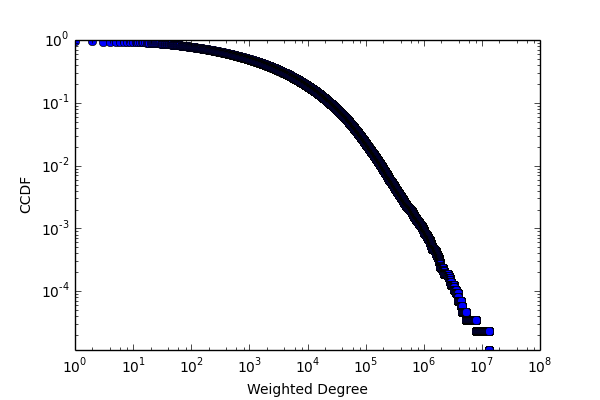
\includegraphics[scale=0.5]{../weighted_degree_ccdf.png}
\caption{CCDF of weighted degree in $\mathcal{G}$}
\label{fig:degree-distribution}
\end{figure}
As stated previously, the weight of an edge is an inverse of the distance between venues, which represent the strength of association between two venues. Then weighted degree is how strongly a venue is associated with all the other venues, therefore shows the relevance of a venue. The power law behaviour seen as the straight line in Figure \ref{fig:degree-distribution} shows that the relevance of venues is largely heterogeneous and could be explained by rich-get-richer model. Indeed, it is perfectly plausible that the higher the relevance of a venue is, the more people visit the location.

One may say that the total number of check-in represents the popularity of a venue. Expectedly, this also exhibits the power law distribution as can be seen in Figure \ref{fig:checkin-distribution}, which is CCDF of the proportion of nodes whose total check-in count is larger than the given count.
\begin{figure}
\centering
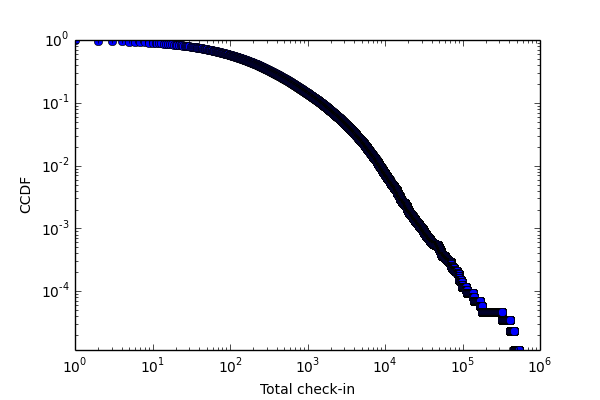
\includegraphics[scale=0.5]{../checkin_new_ccdf.png}
\caption{CCDF of total check-in counts in $\mathcal{G}$}
\label{fig:checkin-distribution}
\end{figure}

Relevance and popularity seems to be two concepts that could be related somehow. Unfortunately the data says otherwise. Each point in Figure \ref{fig:rel-pop} and Figure \ref{fig:rel-pop-zoomed-in} represents a venue in Foursquare dataset, where the latter only shows the venue with fewer than 5000 check-ins. There does not seem to be any clear correlation between two metrics.

\begin{figure}
\centering
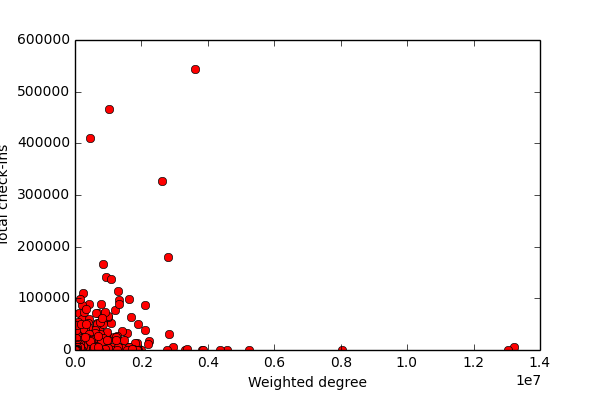
\includegraphics[scale=0.5]{../rel_pop.png}
\caption{Relation between weighted degree and total check-in counts}
\label{fig:rel-pop}
\end{figure}
\begin{figure}
\centering
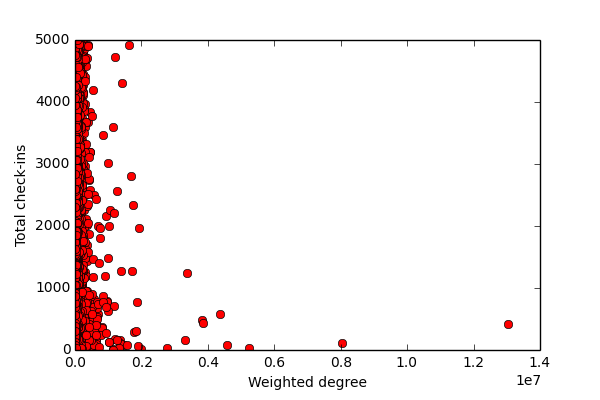
\includegraphics[scale=0.5]{../rel_pop_5000.png}
\caption{Relation between weighted degree and total check-in counts for venues with fewer than 5000 check-ins}
\label{fig:rel-pop-zoomed-in}
\end{figure}

\subsection{Weight distribution}
Recall that we defined the weight of the edge to be an inverse of the distance between two nodes which it connects.
Since distance is much more intuitive metric to consider, we look at the distribution of the inverse of the weight (i.e. distance) in this section.
Figure \ref{fig:distance-ccdf} shows the CCDF of the proportion of nodes whose distance is larger than the given distance, and Figure \ref{fig:distance-distribution} shows the frequency distribution of the distance.
\color{red} We can interpreted these graphs to show the relationship between the distance and the likeliness of checking in. \color{black}
Unlike the total check-in counts or the degree which follows the power law distribution, it shows an exponential distribution with a faster decaying tail.
This is perhaps due to the fact that the check-ins in the dataset are limited to ones in New York, which imposes an upper limit.
\begin{figure}
\centering
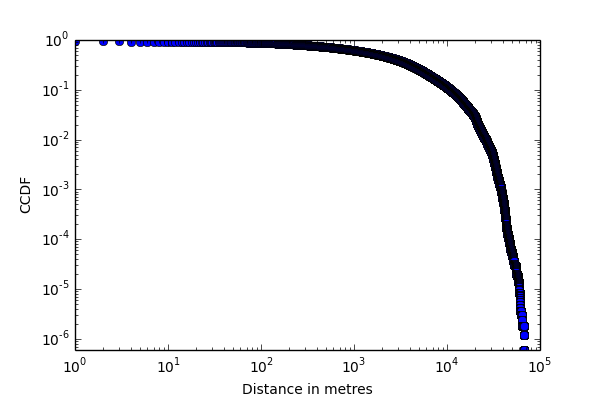
\includegraphics[scale=0.5]{../distance_metres_ccdf.png}
\caption{CCDF of the distance of the transition}
\label{fig:distance-ccdf}
\end{figure}
\begin{figure}
\centering
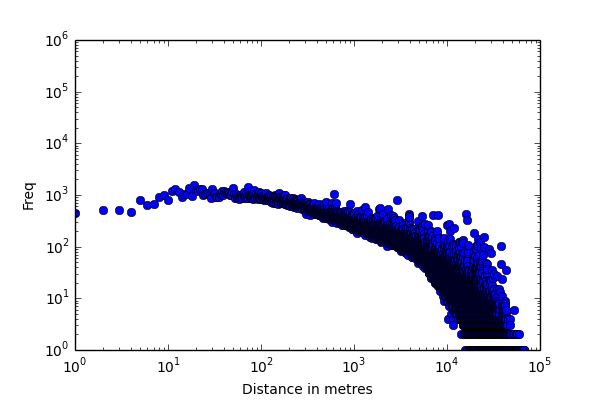
\includegraphics[scale=0.5]{../distance_metres_distribution.png}
\caption{Distribution of the distance of the transition}
\label{fig:distance-distribution}
\end{figure}
\subsection{Clustering Coefficient}
A generalised clustering coefficient for weighted graph was prorposed by \cite{saramaki2007generalizations}. A weighted graph can be translated into a fully connected graph, where the edge that does not exist in the original graph bear zero weight. This gives the notion of \emph{intensity} of a subgraph $g$ with a set of edges $e_{g}$ and a set of nodes $n_{g}$ \citep{saramaki2007generalizations}:
\begin{align*}
I(g) = \left( \prod_{(i, j)\in e_{g}}^{}w_{i, j} \right)^{\frac{1}{|e_{g}|}}
\end{align*}
An unweighted graph can be regarded as a weighted graph where all the edges bear a constant weight therefore the intensity of any triangle is constant. This can be generalised using intensity to obtain the clustering coefficient of a node $i$ as follows\citep{saramaki2007generalizations}:
\begin{align*}
C_i = \frac{2}{(k_i(k_i-1)}\sum_{j, k}^{}(\widetilde{w}_{i, j}\widetilde{w}_{j, k}\widetilde{w}_{k, i})^{\frac{1}{3}}
\end{align*}
where $\widetilde{w}_{i, j}$ is a weight of the edge between $i$ and $j$ normalised with respect to the largest weight of a edge in the network. 
The clustering coefficient of $\mathcal{G}$ is $7.99\mathrm{e}{-5}$ which is very low. This is perhaps is because many triangles include at least one edge with very low weight, which pulls down the intensity of the triangle.
The clustering coefficient of an unweighted graph $\mathcal{G}_u$, which has the same edges and nodes as $\mathcal{G}$ is $0.135$. This is significantly higher than the clustering coefficient of an unweighted random graph $2.85\mathrm{e}{-4}$with the same number of nodes and the average degree as $\mathcal{G}_u$. The clustering coefficient of  $\mathcal{G}_u$ can be interpreted as the transitivity of the existence of association. In other words, it quantifies the extent to which venue A and C are visited in succession if venue A and B, and venue B and C are visited one after the other.
\color{red}average path length \color{black}

\section{Community}
\label{sec:community}
%Especially in a large city there is a certain notion of \emph{neighbourhood}. The notion of neighbourhood is usually somewhat fuzzy, and often there is no well-defined geographical border between them. However, people do seem to have a general consensus on which venue belongs to which area. I argue that the notion of neighbourhood can be defined in terms of the association between venues. For instance, one neighbourhood where the majority of the population belongs to a certain socio-economic group would have many stores or restaurants which are well supported by such a group. We can say that these stores and restaurants should have a strong association among each other. Then, conversely,
Assuming that the edge in $\mathcal{G}$ indeed models the association between venues, we can regard a community in $\mathcal{G}$ as a neighbourhood. We then see whether this definition of neighbourhood mined from $\mathcal{G}$, which I refer to as \emph{Foursquare neighbourhood} corresponds to neighbourhood defined by Airbnb, which I refer to as \emph{Airbnb neighbourhood}. 
\subsection{Extracting Foursquare Neighbourhood}
In order to detect the community in $\mathcal{G}$, I used community detection module \citep{community} which implements the louvain method proposed by \cite{lambiotte2008geographical}. This resulted to 4687 communities. Many consists of a very small number of venues, which are not big enough to be called a neighbourhood. In order to avoid the noise introduced by them, I filtered out the communities with fewer than 1000 venues. This resulted to 30 communities, which we use as Foursquare neighbourhoods. Figure \ref{fig:fsq-comm} shows Foursquare venues coloured according to the Foursquare neighbourhood they belong to. As can be seen, most of the venues which are geographically located closely to each other are in the same community, as the edge that connect them tend to have a higher weight. We can also observe some exceptions. These venue perhaps have at least one edge bearing a high weight with a venue that is geographically far, because there are multiple transitions between them. 
\begin{figure}
\centering
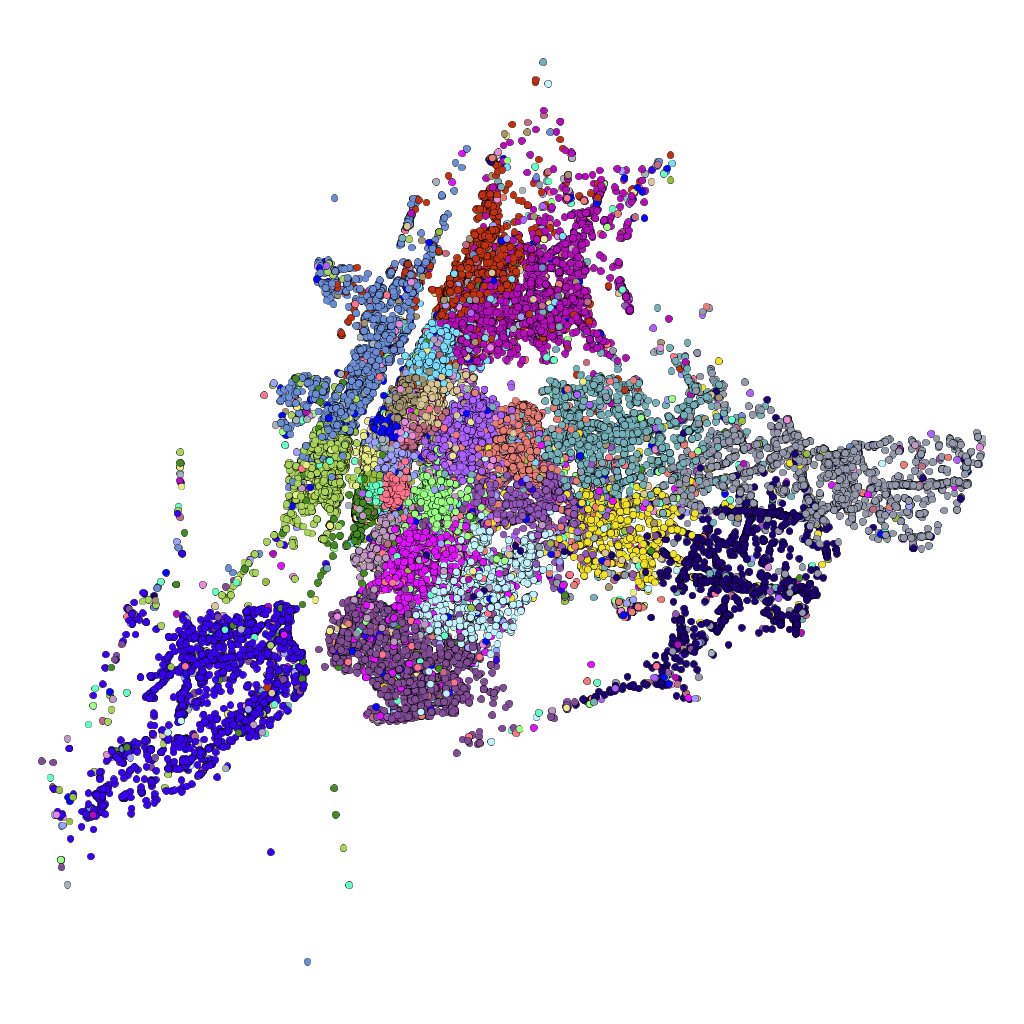
\includegraphics[width=\columnwidth]{../fsq_foo_2.png}
\caption{Foursquare Venues Coloured According to the Foursquare Neighbourhood}
\label{fig:fsq-comm}
\end{figure}
\subsection{Foursquare neighbourhood for Airbnb Listing}
%I assign on each Airbnb listing the same Foursquare neighbourhood that the closest Foursquare venue to the listing belongs to. This is admittedly a very simple measure. Alternatively, one could consider multiple closest Foursquare venues and take the majority.
To draw a comparison between Foursquare neighbourhoods and Airbnb neighbourhoods, I assign a Foursquare neighbourhood on each listing. This section describes the procedure.
Let
\begin{align*}
S(l, n_{fsq}) = S(n_{fsq}) \cap k\_closest\_fsq(l, k)
\end{align*}
where $S(n_{fsq})$ returns a set of Foursquare venues which belong to a Foursquare neighbourhood $n_{fsq}$, and $k\_closest\_fsq(l, k)$ returns $k$ Foursquare venues which are closest to $l$. For a given Airbnb listing, I assign $n_{fsq}$ such that:
\begin{align*}
assign\_fsq\_nbh(l) = \argmax_{n_{fsq}} score(l, n_{fsq})
\end{align*}
where
\begin{align*}
score(l, n_{fsq}) =  \sum_{v \in S(l, n_{fsq})}distance(l, v)^{-1}
\end{align*}
Figure \ref{fig:abnb-comm} shows the Airbnb listings coloured according to the Foursquare neighbourhood they were assigned to, and Figure \ref{fig:abnb-nbh} shows the listings coloured according to the Airbnb neighbourhood they belong to. The colour used for each Foursquare neighbourhood is the same for both Figure \ref{fig:fsq-comm} and Figure \ref{fig:abnb-comm}. Note that Airbnb listings span over a much smaller region, which is why these figures look largely different from Figure \ref{fig:fsq-comm}. Namely, Figure \ref{fig:fsq-comm} includes the west bank of Hudson River. 
\begin{figure}
\centering
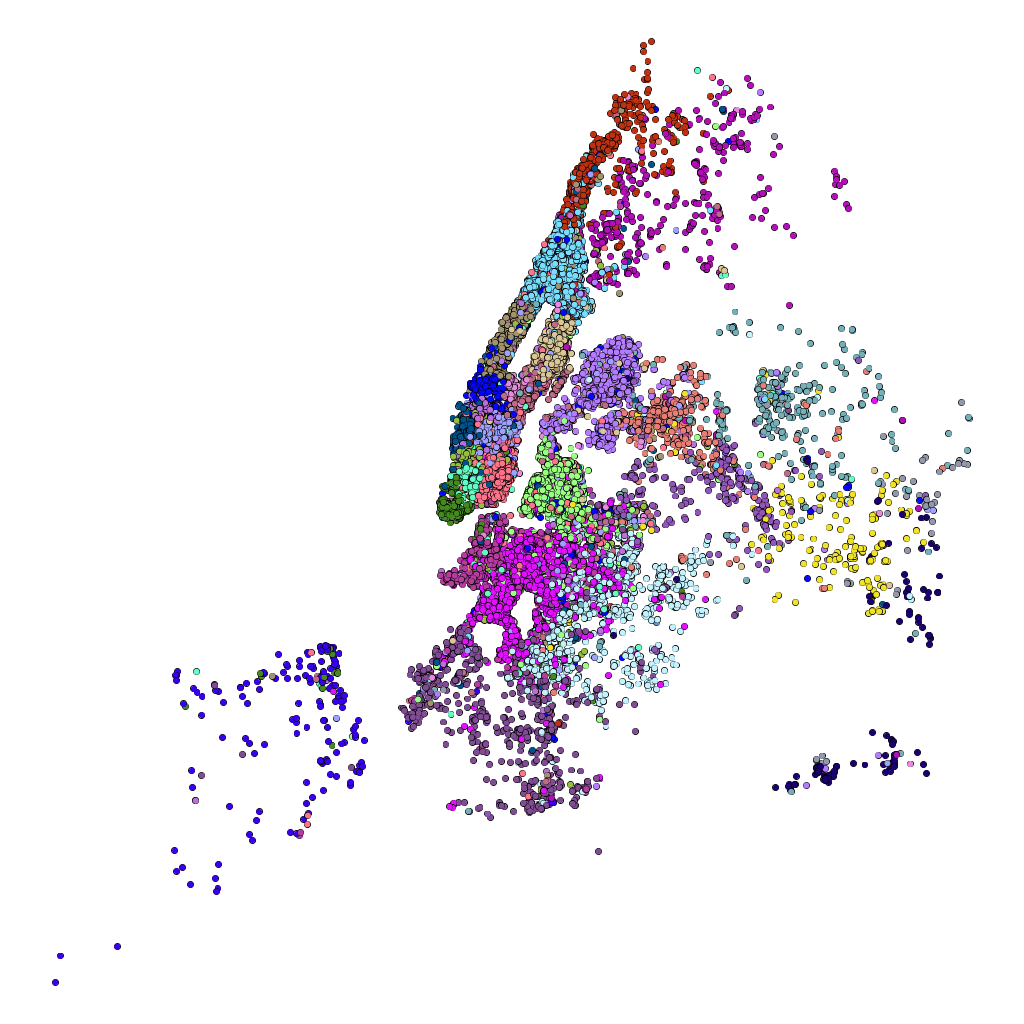
\includegraphics[width=\columnwidth]{../foo_3.png}
\caption{Airbnb Listings Coloured According to Their Foursquare Neighbourhood}
\label{fig:abnb-comm}
\end{figure}
\begin{figure}
\centering
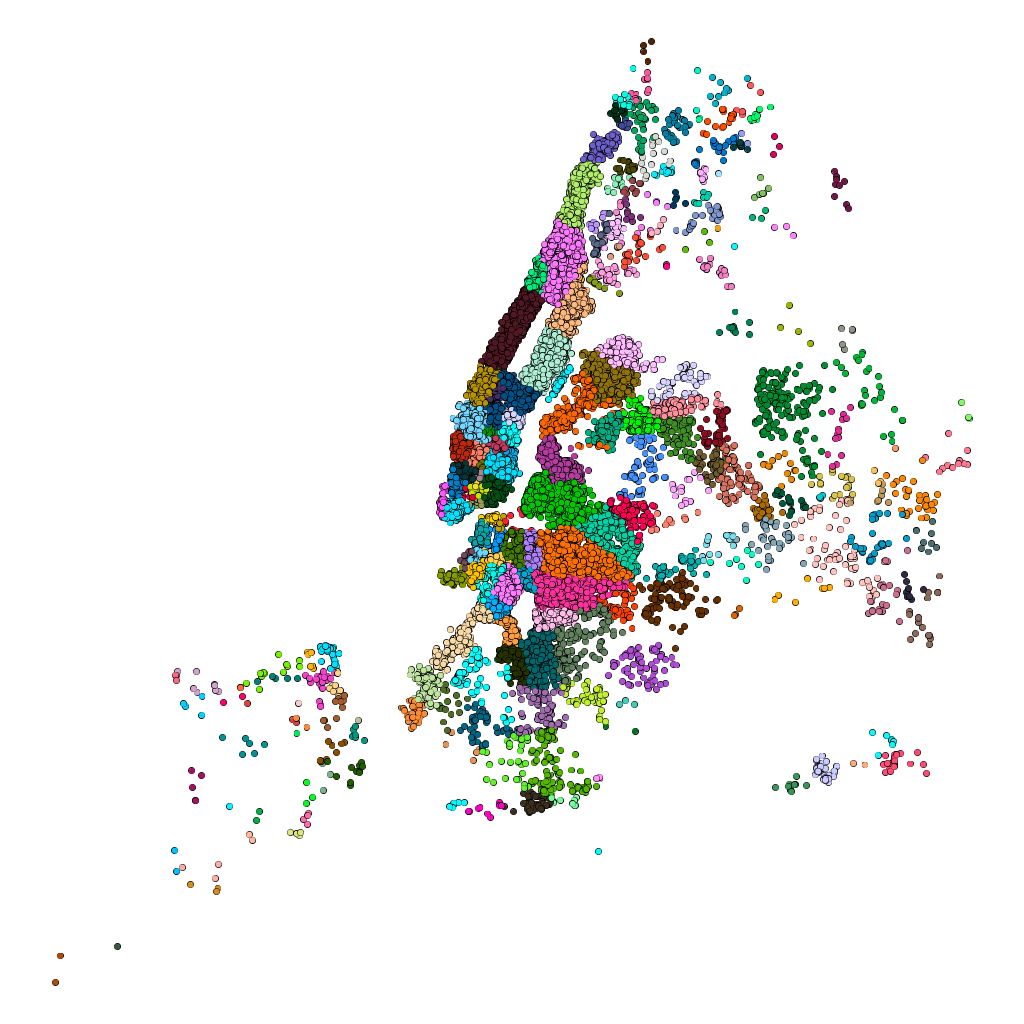
\includegraphics[width=\columnwidth]{../nbh_foo.png}
\caption{Airbnb Listings Coloured According to Their Airbnb Neighbourhood}
\label{fig:abnb-nbh}
\end{figure}
\subsection{Comparing Two Definitions}
First observation one can make is that the Airbnb neighbourhood is more fine-grained with 230 neighbourhoods than the Foursquare neighbourhood with 30 neighbourhoods. This is not due to the threshold value of 1000 venues that I used to filter the neighbourhoods. With the threshold of 1 venue, there would have been 180 neighbourhoods which are already fewer than the number of the Airbnb neighbourhoods. This may though be related to the rate of the decay of the weight with respect to the distance. For instance, if I chose to define $w_{i, j}$ to be inversely proportionate to $distance(i, j)^2$, the Foursquare neighbourhood potentially would have been more fine-grained.

One can say that these two definitions have a high overlap if a given Foursquare neighbourhood groups up multiple entire Airbnb neighbourhoods without splitting them. To quantify the overlap, I first assigned on each Airbnb neighbourhood a Foursquare neighbourhood to which the highest number of its listings were assigned to:
\begin{align*}
&assign\_fsq\_nbh(n_{a}) = \\
&\argmax_{n_fsq} | \{ l | l \in listings(n_{a}), assign\_fsq\_nbh(l) = n_{fsq}\} |
\end{align*}
where $listings(n_{a})$ returns a set of Airbnb listings which belong to $n_{a}$. Then I computed $overlap$ for the set of all the Airbnb listings $S_a$:
\begin{align*}
&overlap(S_a) = \\
& \frac{|\{ assign\_fsq\_nbh(l) = assign\_fsq\_nbh(nbh\_a(l)) | l \in S_a \}|}{|S_a|}
\end{align*}
where $nbh\_a(l)$ returns the Airbnb neighbourhood that $l$ belongs to.

As a result, I found that $overlap(S_a) = 0.653$, which is considerably higher than $3.33\mathrm{e}{-02}$ which what it would have been if a Foursquare neighbourhood was assigned at random on a listing. From this, we can conclude that Foursquare neighbourhood is such that it groups multiple Airbnb neighbourhoods and two definitions of neighbourhood somewhat overlaps.
\section{Popularity}
%The total number of check-in is an indicator of the popularity of a Foursquare venue~\citep{noulas2011empirical}. One may consider an area to be a large Foursquare venue and naturally quantify its popularity as a sum of the number of check-in for Foursquare venues which belong to it. 
As stated previously, the sum of the number of check-ins for Foursquare venues which belong to an area may quantify the popularity of the area. Let this measure of popularity of an area $n$ be $p_{fsq}(n)$.

%On the contrary, there is no agreed way to quantify the popularity of an area using the information about Airbnb listings. 
I first propose various statistics on a set of Airbnb listing that could model the popularity. Then I evaluate its relevance by measuring the correlation with $p_{fsq}$.
\subsection{Candidate Statistics}
Intuitively, a listing is popular if there is more activity; that is, if it is occupied more frequently. Unfortunately, the Airbnb dataset does not offer such information. In the previous works, the activity of a listing was estimated by the number of reviews per month~\citep{cansoy2016gets, insideairbnb}. Airbnb guests may leave a review after their stay. Although it is optional and therefore not all the guests do so, this may be used as an indicator of Airbnb activity. 

Another possible indicator of the popularity of a listing would be the monthly income it generates. Again, this information is not available from the dataset. In the previous works, the minimum income per month was used instead. This can be computed as the product of the minimum length of stay, price and the reviews per month~\citep{cansoy2016gets, insideairbnb}. 

I propose the following statistics to measure the popularity of an area:
\begin{enumerate}
\item $p_{a1}(n)$\\ Average number of reviews per month given to the listings in an area $n$
\item $p_{a2}(n)$\\ Total number of reviews per month given to the listings in an area $n$
\item $p_{a3}(n)$\\ Average minimum income per month among the listings in an area $n$
\item $p_{a4}(n)$\\ Total minimum income per month earned by all the listings in an area $n$
\end{enumerate}
\label{sec:pop-measure}
\subsection{Results}
Figure \ref{fig:checkin_avg_reviews}, \ref{fig:checkin_ttl_reviews}, \ref{fig:checkin_avg_min_income} and \ref{fig:checkin_ttl_min_income} are scatter plots where each point represents a Foursquare neighbourhood. The x-coordinate represents its total check-in counts for the venues and the y-coordinate represents the respective candidate metric proposed in \ref{sec:pop-measure}.

There is no clear correlation between $p_{a1}(n)$ that can be read from Figure \ref{fig:checkin_avg_reviews}. The other statistics, though heteroskedastic, suggest a linear correlation with $p_{fsq}(n)$.

Table \ref{tab:pop-corr} shows Pearson's correlation coefficient $r$ and p-value $p$ between each candidate proposed in \ref{sec:pop-measure} and $p_{fsq}$.
Taking the threshold value of 0.01, only $p_{a3}$ and $p_{a4}$ are significantly correlated to $p_{fsq}$. From this we can conclude that a good statistic which can be obtained from the Airbnb dataset to measure the popularity of an area is either $p_{a3}$ or $p_{a4}$, though the lower p-value for $p_{a3}$ suggests that $p_{a3}$ is a better statistic for this purpose, assuming that $p_{fsq}$ is indeed a good measure of the popularity of an area.

There are two possible reason why $p_{a3}$ and $p_{a4}$ are better suited for measuring the popularity of an area than $p_{a1}$ and $p_{a2}$. One is that the number of reviews per month of a listing may be influenced much more than the popularity of the area, such as the demographics or the purpose of the visits of the guests.

Though the minimum income per month is not independent of these factors, as it is after all defined in terms of the number of reviews per month, the noise introduced might be offset by other variables introduced, which are the price and the minimum length of stay, which possibly has a high correlation with $p_{fsq}$.

% THIS LED ME TRY ..
Figure \ref{fig:checkin_avg_price} and \ref{fig:checkin_avg_length} are scatter plots where each point represents a Foursquare neighbourhood. The x-axis is again the total check-in counts of the venues in the neighbourhood and the y-axis is the average price of the and the average minimum length of stay of a listing, respectively. Unsurprisingly, the average minimum length of stay seems to be invariant of $p_{fsq}$. The average price though seems to have a linear correlation with $p_{fsq}$.  Indeed Pearson's correlation coefficient between the average price and $p_{fsq}$ is $0.742$ with p-value of $ 2.68\mathrm{e}{-06}$, which is lower than that of $p_{a4}$. 
From this we can conclude that the average price of the listing is the best indicator of the popularity of the area. This result goes well with the intuition that a guest would be willing to pay more to be in a popular area.

\begin{figure}
\centering
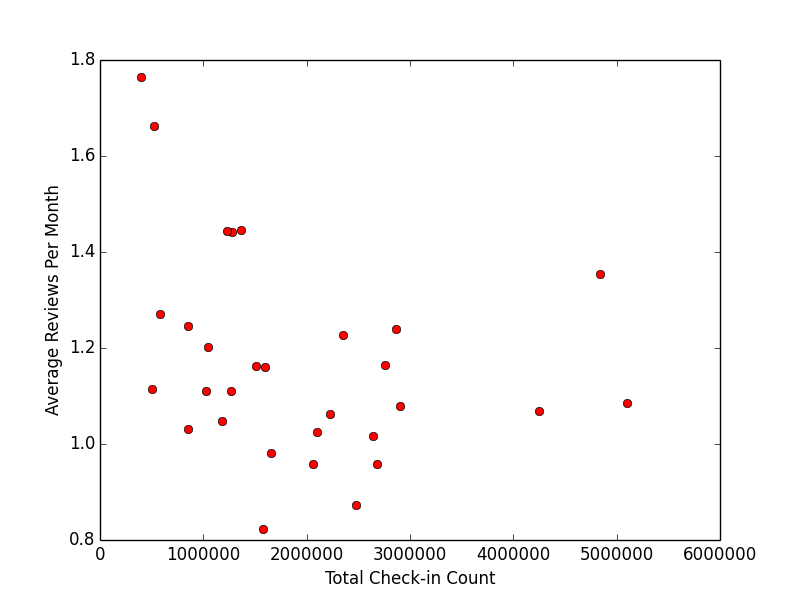
\includegraphics[width=\columnwidth]{../checkin_avg_reviews.png}
\caption{Total Check-in Count and Average Reviews Per Month of Foursquare Neighbourhoods ($p_{a1}(n)$ against $p_{fsq}(n)$)}
\label{fig:checkin_avg_reviews}
\end{figure}
\begin{figure}
\centering
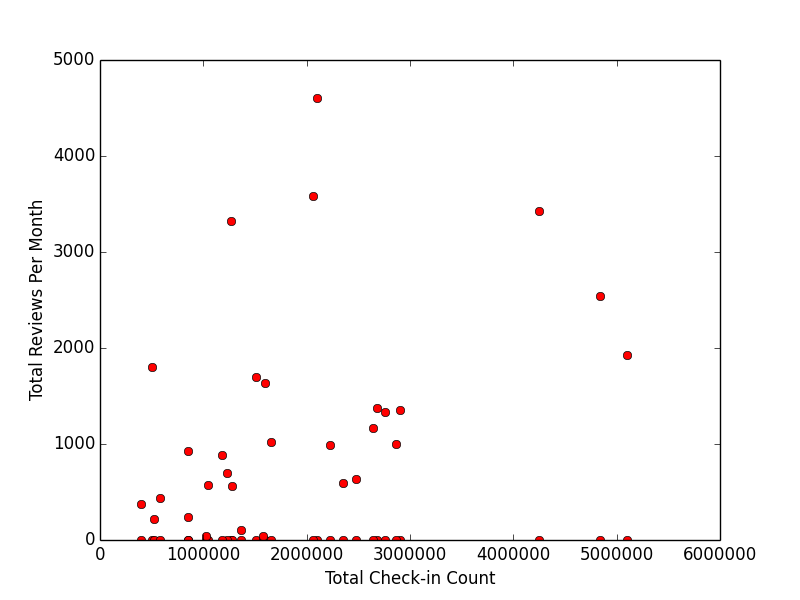
\includegraphics[width=\columnwidth]{../checkin_ttl_reviews.png}
\caption{Total Check-in Count and Total Reviews Per Month of Foursquare Neighbourhoods ($p_{a2}(n)$ against $p_{fsq}(n)$)}
\label{fig:checkin_ttl_reviews}
\end{figure}
\begin{figure}
\centering
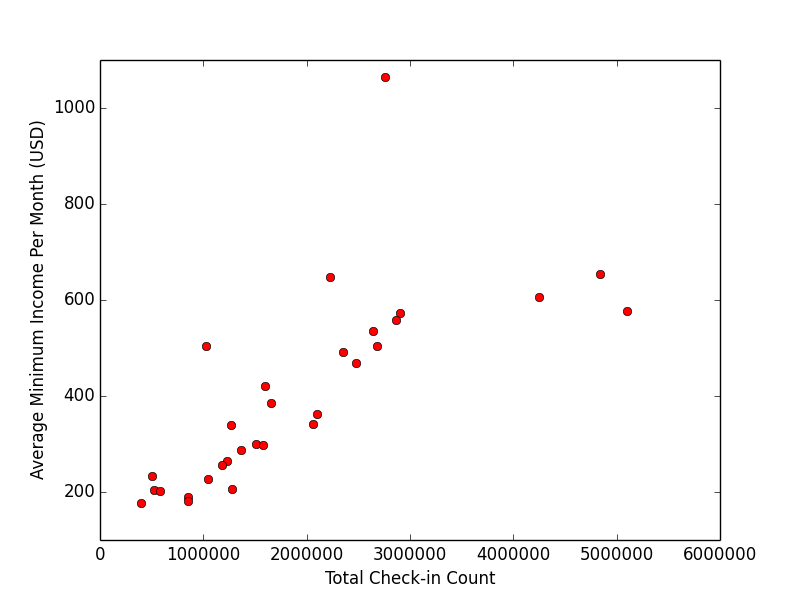
\includegraphics[width=\columnwidth]{../checkin_avg_min_income.png}
\caption{Total Check-in Count and Average Minimum Income Per Month of Foursquare Neighbourhoods ($p_{a3}(n)$ against $p_{fsq}(n)$))} 
\label{fig:checkin_avg_min_income}
\end{figure}
\begin{figure}
\centering
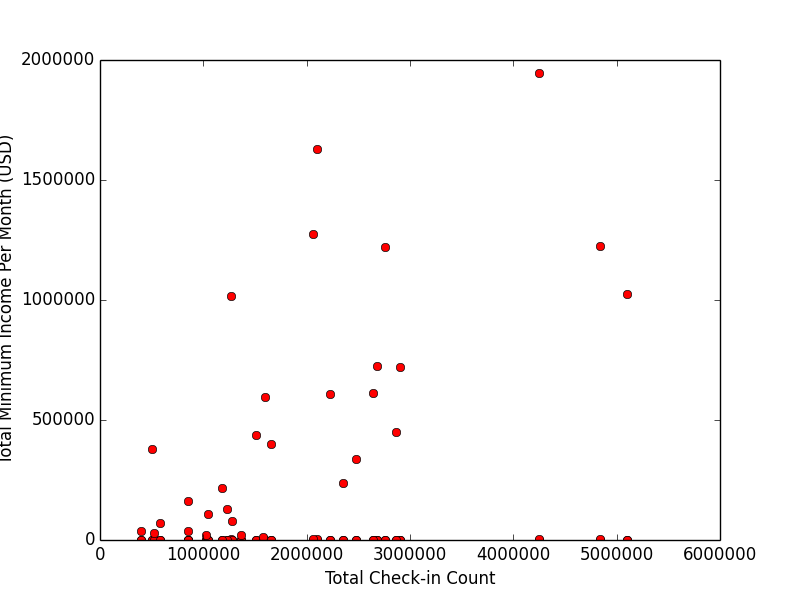
\includegraphics[width=\columnwidth]{../checkin_ttl_min_income.png}
\caption{Total Check-in Count and Total Minimum Income Per Month of Foursquare Neighbourhoods ($p_{a4}(n)$ against $p_{fsq}(n)$)}
\label{fig:checkin_ttl_min_income}
\end{figure}
\begin{table}[]
\centering
\caption{Pearson's Correlation Coefficient $r$ and p-value $p$}
\label{tab:pop-corr}
\begin{tabular}{|l|l|l|}
\hline
         & $r$ & $p$ \\ \hline
$p_{a2}$ &  0.439 & $1.53\mathrm{e}{-02}$     \\ \hline
$p_{a3}$ &  0.728   & $5.07\mathrm{e}{-06}$  \\ \hline
$p_{a4}$ & 0.697 & $1.88\mathrm{e}{-05}$     \\ \hline
\end{tabular}
\end{table}
\begin{figure}
\centering
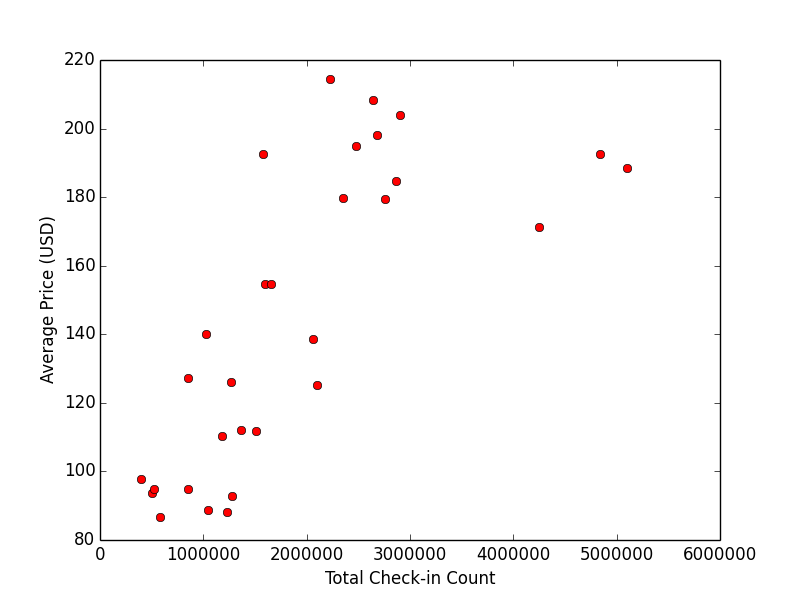
\includegraphics[width=\columnwidth]{../checkin_avg_price.png}
\caption{Total Check-in Count and Average Price of Listings in Foursquare Neighbourhoods}
\label{fig:checkin_avg_price}
\end{figure}
\begin{figure}
\centering
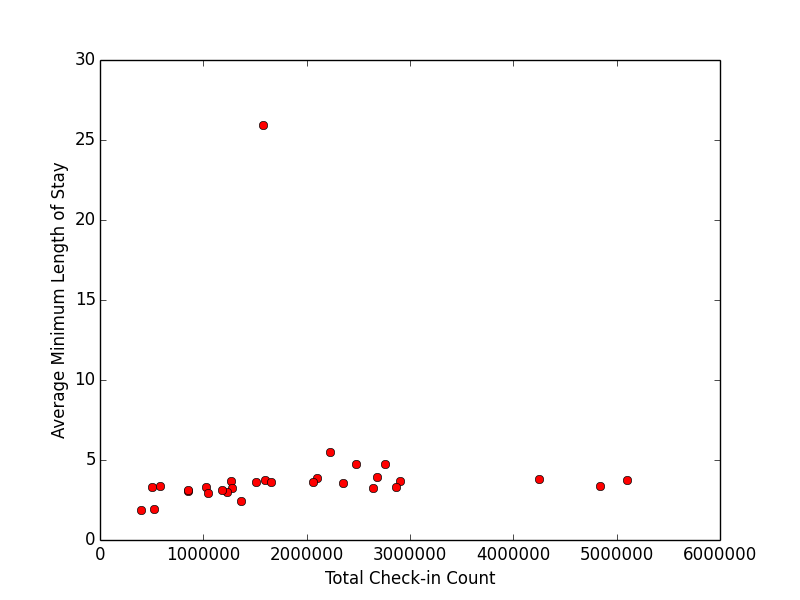
\includegraphics[width=\columnwidth]{../checkin_avg_length.png}
\caption{Total Check-in Count and Average Minimum Length of Stay of Listings in Foursquare Neighbourhoods}
\label{fig:checkin_avg_length}
\end{figure}

\section{Discussion}
\label{sec:discussion}
One factor that was not taken into account is the time elapsed since the first check-in till the second check-in in the transition. \cite{noulas2011empirical} states that two temporally close check-ins of the same user could signal an important correlation between
two locations, but as this temporal distance increases we could express higher confidence that the two check-ins are not strictly consequential. \cite{noulas2011empirical} though also demonstrates that there is a positive correlation between inter-check-in times and inter-check-in distances. This means that two check-ins made with a long interval may still be strongly related if they are located further away from each other. As a future work, one may create a more elaborate model for the strength of association by taking such factors into account, which may lead to a better definition of Foursquare neighbourhoods.

We made an assumption that the total check-ins of the venues in an area is an adequate indicator of its popularity. One may investigate a potential bias of this statistic by considering for instance the demographics of the users of Foursquare.

% include your own bib file like this:
\bibliography{l109}
\nocite{*}
\bibliographystyle{plainnat}



\end{document}